\subsection{Git (Mikkel)}
We used Git as a the primary version control tool in order to have multiple groups of people implementing code simultaneously. As we primarily worked in pairs this meant we doubled our effectiveness by handling two problems at the same time. In order to achieve this, we had a routine of \textit{"Branch - Work - Merge"} once a day, if not more. One such occurrence can be seen in the figure below.

\begin{figure}[H]
    \centering
    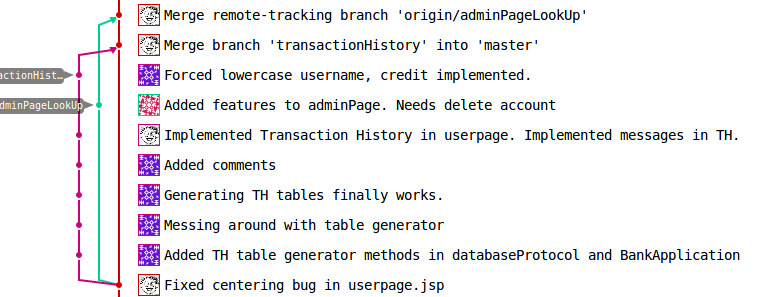
\includegraphics[width=\linewidth]{figures/git.png}
    \caption{An example of branching in the Git-commit timeline.}
    \label{fig:git}
\end{figure}


%how we used git. network figure, commit history figure.